\documentclass[11pt,letterpaper]{article}
\usepackage[utf8]{inputenc}
\usepackage{geometry}
\usepackage{blindtext}
\usepackage{amsmath}
\usepackage{amssymb}
\usepackage{multicol}
\usepackage{gensymb}
\usepackage{tikz}
\usepackage{pgfplots}
\usepackage{pgfplotstable}
\pgfplotsset{compat = newest}
\usepackage{fancyhdr}

\pagestyle{fancy}
\fancyhf{}
\rhead{\small {© 2022 All Rights Reserved, Aiden Rosenberg}}
\rfoot{Page \thepage}

\title{A.P Physics Pendulum Lab  }
\author{Aiden Rosenberg \\ \\ Period: 5th }
\date{Thu March 3 2022 A.D}

\begin{document}
\maketitle 


\pagebreak
\section{Introduction}

\subsection{Propose}
To determine an experimental value for gravity using observations of simple harmonic motion  

\subsection{Hypothesis}
Observing the relationship between length and period of a simple pendulum, we will determine that gravity has a value of $9.8 \frac{m}{s^2}$.

\begin{figure}
    \centering
  \includegraphics[width=0.5\linewidth]{Apparatus .png} 
    \caption{Pendulum Diagram}
    \label{fig:my_label}
\end{figure}


\subsection{Materials}

\begin{enumerate}
    \item One Lab stand
    \item 40 cm of string
    \item Small mass with a hook or eye (approx 100g) 
    \item One stopwatch 
    \item One slow motion camera
    \item One metre-stick
    \end{enumerate}
\pagebreak
\section{Procedure}
\begin{enumerate}
    \item Cut a 40cm piece of string and tie a loop at both ends of the string.
    \item Attach the segment of sting to the horizontal cross member of the lab stand by using the previously created loops. 
    \item Hook a mass of approx 100g to the opposite end of the string so that the mass creates tension in the string.  
    \item Measure the distance from the centre of mass of the attached mass and recorded. Use the recorded length to calculate result of the equation $4\pi^2l$.
    \item Gently pull the mass away from equilibrium until the centre of mass reaches a maximum of $\theta \lessapprox \frac{\pi}{12}$. Reference to figure 1.
    \item Start a stopwatch and begin filming with slow mo camera so that the stopwatch is in the video frame.
    \item Release the mass from $\theta \lessapprox \frac{\pi}{12}$ and film the oscillations for 2 or more periods (time it takes the mass to traverse from $\theta \lessapprox \frac{\pi}{12}$ to $-\theta \lessapprox \frac{\pi}{12}$ and back to $\theta \lessapprox \frac{\pi}{12}$ ).
\begin{enumerate}
    \item $\theta \lessapprox \frac{\pi}{12} \Longleftrightarrow \theta \lessapprox 15^{\circ}$
\end{enumerate}
    \item Analyse the camera footage frame by frame using the time on the stopwatch as a reference to calculate the period of the mass. Start by finding the recorded time $t_{1}$ at the instant the mass is released from $\theta \lessapprox \frac{\pi}{12}$. Next traverse footage until the mass returnees to $\theta \lessapprox \frac{\pi}{12}$ and find the displayed time $t_{2}$. Using the following equation to calculate the period $T_{p}=t_{2}-t_{1}$ and recorded. 
    \item Repeat steps 5-8 for three trials and use the subsequent recorded measurements to calculate the average period across each trial. $T_{avg}=\frac{\Sigma T_{p}}{3}$
    \item For each trial calculate $T_{p}^2$ and recorded.  
    \item Repeat steps 3-10 for four trials, each decreasing the length of the string each time.
    \item Graph $\frac{\mathrm d (4\pi^2l) }{\mathrm d (T_{p}^2)}$, using the data points of ($T_{p}^2, 4\pi^2$) for each trial and use liner aggression to draw a trend line. Check if the slope of the trend line is equal to gravitation acceleration.  

    \end{enumerate}
    \pagebreak
\section{Data Table}

\begin{table} [h]
\begin{tabular}{rrrrrrr}
\multicolumn{1}{l}{\textbf{}}                       & \multicolumn{3}{l}{\textbf{Times for 1 oscillation [s]}}                                                                & \multicolumn{1}{l}{\textbf{}}                    & \multicolumn{2}{l}{\textbf{Graphical Data}}                                              \\ \hline
\multicolumn{1}{|l|}{\textbf{Length of string [m]}} & \multicolumn{1}{l|}{\textbf{Trial 1}} & \multicolumn{1}{l|}{\textbf{Trial 2}} & \multicolumn{1}{l|}{\textbf{Trial 3}} & \multicolumn{1}{l|}{\textbf{$T_{avg}^2$ [s]}} & \multicolumn{1}{l|}{\textbf{$T_{P}$ [s]}} & \multicolumn{1}{l|}{\textbf{$4 \pi^2l$ [m]}} \\ \hline
\multicolumn{1}{|r|}{0.13}                          & \multicolumn{1}{r|}{0.67}             & \multicolumn{1}{r|}{0.66}             & \multicolumn{1}{r|}{0.65}             & \multicolumn{1}{r|}{0.66}                        & \multicolumn{1}{r|}{0.4356}      & \multicolumn{1}{r|}{5.1321}                           \\ \hline
\multicolumn{1}{|r|}{0.24}                          & \multicolumn{1}{r|}{0.94}             & \multicolumn{1}{r|}{0.89}             & \multicolumn{1}{r|}{0.92}             & \multicolumn{1}{r|}{0.9166666667}                & \multicolumn{1}{r|}{0.84026}     & \multicolumn{1}{r|}{9.4748}                           \\ \hline
\multicolumn{1}{|r|}{0.33}                          & \multicolumn{1}{r|}{1.13}             & \multicolumn{1}{r|}{1.16}             & \multicolumn{1}{r|}{1.11}             & \multicolumn{1}{r|}{1.133333333}                 & \multicolumn{1}{r|}{1.28443}     & \multicolumn{1}{r|}{13.0278}                          \\ \hline
\multicolumn{1}{|r|}{0.49}                          & \multicolumn{1}{r|}{1.38}             & \multicolumn{1}{r|}{1.41}             & \multicolumn{1}{r|}{1.39}             & \multicolumn{1}{r|}{1.393333333}                 & \multicolumn{1}{r|}{1.9413}      & \multicolumn{1}{r|}{19.3444}                          \\ \hline
\end{tabular}
\end{table}
\textit{Collected for each trial with derived mathematical values}
\section {Graph}
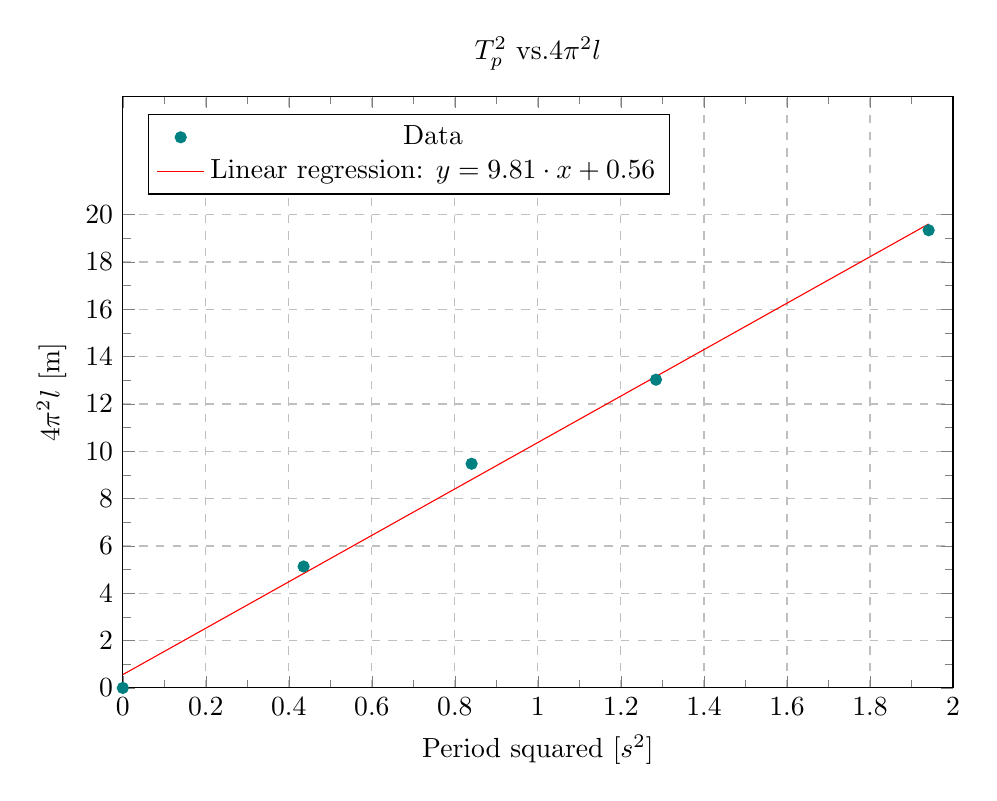
\begin{tikzpicture}
        \begin{axis}[
          title={$T_{p}^2$ vs.$4 \pi^2l$},
          xlabel={Period squared [$s^2$]},
          ylabel={ $4 \pi^2l$ [m]},
          xmin=0, xmax=2,
          ymin=0, ymax=25,
          xtick={0,0.2,0.4,0.6,0.8,1,1.2,1.4,1.6,1.8, 2},
          ytick={0,2,4,6,8,10,12,14,16,18,20},
          legend pos=north west,
            ymajorgrids=true,
            xmajorgrids=true,
            grid style=dashed,
            minor tick num = 1,
            major grid style = {lightgray},
            minor grid style = {lightgray!25},
            width = \textwidth,
            height = 0.75\textwidth
        ]
   \addplot[teal, only marks] table[row sep=\\]{
        X Y\\
        0 0\\
        0.4356 5.1321\\
        0.84026 9.4748\\
        1.28443 13.0278\\
        1.9413 19.3444\\
        };
     
    \addplot [red, no marks] table[row sep=\\,
    y={create col/linear regression={y=Y}}] 
    {
        X Y\\
        0 0\\
        0.4356 5.1321\\
        0.84026 9.4748\\
        1.28443 13.0278\\
        1.9413 19.3444\\
    };
    
            \addlegendentry{Data}
            \addlegendentry{
                Linear regression:
                $
                y =
                \pgfmathprintnumber{\pgfplotstableregressiona}
                \cdot x
                \pgfmathprintnumber[print sign]{\pgfplotstableregressionb}
                $
            };
        \end{axis}
    \end{tikzpicture}
\\If graphed by hand $\Rightarrow g=\frac{y_{2}-y_{1}}{x_{2}-x_{1}} \approx 10\frac{m}{s^2} $
\section{Calculations}
\subsection{Example Calculations (\textit {$l = 0.13m$})}
$T:$ Period \\ $l:$ sting length\\
$$T_{P}=2\pi \sqrt{\frac{l}{g}} \Longleftrightarrow g \propto \frac{4\pi ^2}{T_{P}^2l}$$
\begin{enumerate}
   \item $T_{p} = t_{2}-t_{1}$ : \textit {Calculate the time interval}
    \item $T_{avg}=\frac{\Sigma T_{p}}{3} \Rightarrow T_{avg}= \frac{0.67s + 0.66s + 0.65s}{3} \Rightarrow T_{avg} \approx 0.\overline{66}  $: \textit {Calculate the average period across each trial.}
    \item $T_{avg}^2= 0.4356 s^2$
    \item $4 \pi^2 \cdot l \Rightarrow 4 \pi^2 \cdot 0.13m \approx 5.1321m $: \textit { Calculate the period squared }
    \item $ (T_{p}^2, 4\pi^2) \Longrightarrow (0.66, 5,1321)$: \textit {Convert to Cartesian point}
\end{enumerate}
\textit{Repeat these calculations for each trial and fill in the data table}

\subsection{Percent error}
$\delta = \biggr|\frac{v_{A}-v_{E}}{v_{e}}\biggr| \cdot 100 \Rightarrow \delta = \biggr| \frac{9.81\frac{m}{s^2}-9.81\frac{m}{s^2}}{9.81 \frac{m}{s^2}}\biggr| \cdot 100 \Longrightarrow \delta =0 \%$ error
\\ $\delta$: Percent error
\\ $v_{A}$: actual value observed  $\Longrightarrow v_{A}= 9.81 \frac{m}{s^2}$
\\ $v_{E}$: expected value $\Longrightarrow v_{E}= 9.81 \frac{m}{s^2}$ 

\subsection{Free Body Diagram}
\begin{center}
   \includegraphics[width=2in]{FBD.png}
\end{center}
\pagebreak
\section{Conclusion}
In subsequent responses to the results gathered by the Pendulum Lab, affirmed the initial hypothesis with a reasonable degree of accuracy that an experimental value for gravity using observations of simple harmonic motion can be derived. The experiment contained zero percent error, comparing the derivative of the graph function of $\frac{\mathrm d (4\pi^2l) }{\mathrm d (T_{p}^2)} \approx 9.81 \frac{m}{s^2} $; with length as the independent variable, to the gravitational acceleration constant of earth $9.81 \frac{m}{s^2}$. This ratio was derived from the following equation for period of a pendulum via solving for the gravitational acceleration:$$T_{P}=2\pi \sqrt{\frac{l}{g}} \Longleftrightarrow g \propto \frac{4\pi ^2l}{T_{P}^2}$$
The gravitational acceleration g near the surface of the Earth is known to be approximately  ($9.81 \frac{m}{s^2}$) a constant value, disregarding small effects due to geological variations and altitude shifts. The equation above models the period of a a bob with negligible friction and air resistance as attached to a static string, thus eliminating sources of non mechanical energy loss. This equation models an increasing liner relationship whose slope is proportional to $g$.  lab gathered results from a pendulum hung from a horizontal crossbeam by a string of length $l$ with a bob of 200g moved from equilibrium so that $\theta \lessapprox \frac{\pi}{12}$ ; the bob was subsequently released to measure its period. As the mass was released from $\theta \lessapprox \frac{\pi}{12}$ the period of the bob was was filmed digitally using the time stamps of slow mo camera footage to determine the instantaneous difference from $t_{final}$ to $t_{initial}$ thus calculating the period of the pendulum for length $l$. In order to confirm the proportionality in the equation above, four different string lengths were used $l_{1}=0.13m,\ l_{2}=0.24m ,\ l_{3}=0.33m $ \& $l_{4}=0.49m$. For each length the period was record for three trial to reduces possibility of error; the average of each trial was used as the period for the given length. Using the collected data  $\frac{\mathrm d (4\pi^2l) }{\mathrm d (T_{p}^2)}$, was plotted using the data points of ($T_{p}^2, 4\pi^2l$) for each trial and using liner regression to create a trend line. Manipulating the equation above into  the form $y=mx+b \Rightarrow T_{p}^2=4\pi ^2\cdot l +0 $  hence graphing the liner relationship between $T_{p}^2$ \& $ 4\pi^2 \cdot l$  results in a trend line with the following equation; $y = 9.81 ·x + 0.56 \Rightarrow y'=9.8 \frac{m}{s^2}$. 
\\\\ Since the percent error is null there is no deviation between our accepted value, and that of the expected value(A.P approx of $9.8\frac{m}{s^2} $ ) therefore our results our accurate. The results compiled in this lab confirmed our logical reasoning that gravitational acceleration on the earths surface is approximately a constant of $9.8\frac{m}{s^s}$; the relationship between the graph quantities was linear therefore the derivative of the trend line is constant. During the initial completion of this lab the procedure was modified to include steps that used slow motion camera technology and the video graphic timestamps to calculate the period of the bob rather than using a stopwatch to time 10 oscillations.  This lab was also modified to incorporate the use of a computer graphing application which subsequently decreased the percent error by 1.936 \% since the slope of the hand drawn trend line approximately $10 \frac{m}{s^2}$. Although our statistical data confirmed with out any sources of error a corrects numerical value for gravity; the preciseness of our measurements corresponds to the scope of the experiment. In order for more complicated analysis would require the use of photon gates,  a friction less pulley and increased the number of data points for linear regression calculations. This corresponds to the current limitation of this lab; minute number of significant figures, rounding errors and the limitations of classroom technology. Albeit the derivative of the trend line derived was within the zero percent error to the standard approximation of earths gravitational constant it is by is no way the the absolute value of since the sample measurement could have experienced drag and external forces thus deviating minutely from the exact gravitational value.  In conclusion for the scope of the the triviality of the class any possible error is proven null thus we assume the  gravitational acceleration at DHS is approximately $9.8\frac{m}{s^2} $.

\end{document}
